\documentclass[a4paper,12pt]{article}
\usepackage[margin=1in]{geometry}
\usepackage[singlespacing]{setspace}
\usepackage[english]{babel} % Figure captions
\usepackage{mathpazo} % Font
\usepackage{fixltx2e} % Subscript Fix
\usepackage{hyperref} % Subscript Fix
\usepackage{verbatim} % Comment tool
\usepackage{graphicx} % Add images
\usepackage{apacite}
\usepackage{etoolbox}
\usepackage{environ}
\usepackage{sectsty}
\usepackage{gensymb}  % Degree Symbol
\usepackage{textcomp} % Prevents gensymb package warning
\usepackage{listings}
\usepackage{color}


\newenvironment{code}{\fontfamily{cmtt}\selectfont}{\par}

\definecolor{mygreen}{rgb}{0,0.6,0}
\definecolor{mygray}{rgb}{0.5,0.5,0.5}
\definecolor{mymauve}{rgb}{0.58,0,0.82}

\lstset{ %
  backgroundcolor=\color{white},   % choose the background color; you must add \usepackage{color} or \usepackage{xcolor}
  basicstyle=\tiny,        % the size of the fonts that are used for the code
  breakatwhitespace=false,         % sets if automatic breaks should only happen at whitespace
  breaklines=true,                 % sets automatic line breaking
  captionpos=b,                    % sets the caption-position to bottom
  commentstyle=\color{mygreen},    % comment style
  deletekeywords={...},            % if you want to delete keywords from the given language
  escapeinside={\%*}{*)},          % if you want to add LaTeX within your code
  extendedchars=true,              % lets you use non-ASCII characters; for 8-bits encodings only, does not work with UTF-8
  frame=single,                    % adds a frame around the code
  keepspaces=true,                 % keeps spaces in text, useful for keeping indentation of code (possibly needs columns=flexible)
  keywordstyle=\color{blue},       % keyword style
  language=Octave,                 % the language of the code
  otherkeywords={*,...},            % if you want to add more keywords to the set
  numbers=left,                    % where to put the line-numbers; possible values are (none, left, right)
  numbersep=5pt,                   % how far the line-numbers are from the code
  numberstyle=\tiny\color{mygray}, % the style that is used for the line-numbers
  rulecolor=\color{black},         % if not set, the frame-color may be changed on line-breaks within not-black text (e.g. comments (green here))
  showspaces=false,                % show spaces everywhere adding particular underscores; it overrides 'showstringspaces'
  showstringspaces=false,          % underline spaces within strings only
  showtabs=false,                  % show tabs within strings adding particular underscores
  stepnumber=1,                    % the step between two line-numbers. If it's 1, each line will be numbered
  stringstyle=\color{mymauve},     % string literal style
  tabsize=4,                       % sets default tabsize to 2 spaces
  title=\lstname                   % show the filename of files included with \lstinputlisting; also try caption instead of title
}

\AtBeginDocument{
    \let\cite\shortcite %  One-two author and then et al.
    \renewcommand{\BBAY}{ } % Spaces in betweEn in-line citation author-year
    \renewcommand{\BBAA}{and} % And in between two authors instead of &
    \renewcommand{\BOthers}[1]{\textit{et al.}\hbox{}} % et al.
    \renewcommand{\BOthersPeriod}[1]{\textit{et al.}\hbox{}} % et al.
    \renewcommand\refname{\textsc{Literature Cited}} % Change bib header
    \renewcommand{\baselinestretch}{1.9}
}

\newtoggle{bibdoi}
\newtoggle{biburl}
\makeatletter
\undef{\APACrefURL}
\undef{\endAPACrefURL}
\undef{\APACrefDOI}
\undef{\endAPACrefDOI}
\long\def\collect@url#1{\global\def\bib@url{#1}}
\long\def\collect@doi#1{\global\def\bib@doi{#1}}
\newenvironment{APACrefURL}{\global\toggletrue{biburl}
\Collect@Body\collect@url}{\unskip\unskip}
\newenvironment{APACrefDOI}{\global\toggletrue{bibdoi}
\Collect@Body\collect@doi}{}

\AtBeginEnvironment{thebibliography}{
 \pretocmd{\PrintBackRefs}{
  \iftoggle{bibdoi}
    {\iftoggle{biburl}{}{}}
    {\iftoggle{biburl}{}{}}
  \togglefalse{bibdoi}\togglefalse{biburl}
  }{}{}
}

\begin{document}

\lstset{language=R}

%------------------------------------------------------------------------------
% Prompt
%------------------------------------------------------------------------------

\begin{comment}

For the final project, students will write a scientific manuscript based on their proposal that adheres to the format of a Letter for the journal Ecology Letters.
Specifically, the manuscript will have the following structure: “Abstract”, “Introduction”, “Methods & Materials”, “Results”, “Discussion”, “References”, “Tables”, “Figures”; all in no more than 5,000 words and 6 tables/figures.
The manuscript will present a novel model that tackles the topic described in the proposal.
The paper will also include an appendix describing the rationale for the model derivation and analysis, along with the R code used to produce the results.

\end{comment}

%------------------------------------------------------------------------------
% Title Page
%------------------------------------------------------------------------------

\begin{titlepage}

\noindent

\begin{center}

\textbf{Agricultural species diversity to mitigate\\\textit{Aspergillus} crop infection and Aflatoxin B\textsubscript{1} human exposure}

\noindent\textsc{Clint Valentine}

\noindent\textsc{May 1, 2015}

\end{center}

\end{titlepage}

\doublespacing

%------------------------------------------------------------------------------
% Abstract
%------------------------------------------------------------------------------

\section*{\upshape\textsc{Abstract}}

\emph{Aspergillus flavus} is a ubiquitous soil fungus that produces the carcinogenic secondary metabolite aflatoxin B\textsubscript{1} (AFB\textsubscript{1}).
The genus \emph{Aspergillus} is able to infect many primary agricultural food crops in low incidence.
Chronic human consumption of AFB\textsubscript{1} is one of the leading causes of hepatocellular cancer and stunting in children.
The ecology of monocultured crops may lend to higher infection rates of \emph{A. flavus} due to a lack of biodiversity in crops of variable fungal resistance.
We propose a spatially constructed model for simulating crop infection through the dynamics of active spores of \emph{A flavus} (conidia) whereby we can examine the steady state infection rates of the crops in biodiverse settings.

%------------------------------------------------------------------------------
% Introduction
%------------------------------------------------------------------------------

\section*{\upshape\textsc{Introduction}}

The human liver carcinogen aflatoxin B\textsubscript{1} (AFB\textsubscript{1}) is a prevalent secondary metabolite produced by the fungi \emph{Aspergillus flavus} \cite{Groopman2014a}.
AFB\textsubscript{1} has been well studied as the most carcinogenic naturally found compound to the human liver.
\emph{Aspergillus} is also one of the most ubiquitous genus of fungi that is readily isolated from plants, air, soil, and insects \cite{Wicklow2003}.
The toxicity of AFB\textsubscript{1} coupled with the prevalence of \emph{Aspergillus} impacts human health-care and agricultural yield in a large way.
It is estimated that agricultural yield loss due to \emph{Aspergillus} is approximately \$1 billion dollars annually in the United States alone \cite{Robens2003}.
The economic effect of \emph{Aspergillus} contamination is estimated to be more severe in developing nations \cite{Amaike2011}.
Subsequent human exposure of AFB\textsubscript{1} through contamination is especially endemic in developing countries as a result of grain processing, quality control, and storage practices which favor mold growth \cite{Schmidt2013}.

There are an estimated 4.5 billion people in the developing world that are chronically affected by aflatoxins in their diet and these exposures may account for between 25,200 and 155,000 cases of hepatocellular cancer yearly \cite{Liu2010}.
In 2013, a cross-sectional study published in \textit{Food Additives \& Contaminants} shows that approximately 78\% of 3,000 randomly selected serum samples in Kenya had detectable amounts of aflatoxins \cite{Yard2013}.
In the same National Health \& Nutrition survey it was found that approximately 17\% of 2,000 randomly selected serum samples in the United States of America had detectable levels of aflatoxin compounds \cite{Yard2013}.
This contrast shows a need for better agricultural and educational methods to control for aflatoxin exposure in developing nations.

AFB\textsubscript{1} exposure is not only the cause of hepatocellular carcinoma but a myriad of other detrimental health effects.
The link between aflatoxin exposure and childhood stunting was borne from the research of Kitty Cardwell, a plant pathologist with the Department of Agriculture (USDA).
Cardwell compared blood samples from 700 children in her local area of study in Benin and Nigeria with stunting and correlated this health disparity with AFB\textsubscript{1} biomarkers \cite{Gong2002}.
DeOnis \emph{et al.} (2012) estimate 171 million cases of stunting in children worldwide and the proportion of which due to AFB\textsubscript{1} is, at the moment, poorly understood.

Research involving the infection and transmission of \textit{Aspergillus} species is critical in understanding why liver cancer is the third highest incidence cancer globally \cite{Liu2010}.
\textit{Aspergillus} is resilient in most environments between 54\degree{}--118\degree{}C with high oxygen content \cite{Schmidt2013}.
The fungus is most frequently found between latitudes of 16\degree{} and 35\degree{} \cite{Klich2007}.
Crops become susceptible to \textit{Aspergillus} through heat stress, high soil moisture, and insect-induced injury \cite{Amaike2011}.
Protecting crops is a challenge because \textit{Aspergillus} can grow in many nutrient-deprived environments and the conidia can lay dormant within disturbed soil for over three years \cite{Abbas2009}.
Mitigating \textit{Aspergillus} crop infection is further complicated due the difficulty in spotting and removing the infected plants.

It has been shown that genetic diversity within host populations aids in reducing the overall impact of infectious disease.
This natural phenomenon has been shown to exist in many examples including mammals, birds, aquatic invertebrates, and plants \cite{Ostfeld2011}.
Schmidt and Ostfeld first noted that this `dilution effect' of the pathogen can occur when the species richness of an environment is increased \cite{Schmidt2001}.

\emph{Aspergillus flavus} are able to survive on plant residues due to the formation of a life stage morphology called mycelia \cite{Wicklow1993}.
Mycelia or sclerotia of \emph{A. flavus} can reproduce and thrive throughout the detritus and nutrients found in the soil \cite{Abbas2009}.
As mycelia mature they enter a sporulating stage which produce many conidia.
Conidia are then dispersed over large surface areas during the saprophytic life stage due to the forces of wind, rain, and insect travel \cite{Abbas2008}.
Conidia are able to infect agricultural crop through mechanical and chemical interaction and are often aided by insect and bird damage to the crop.
These damages often provide entry sites for the fungus to succeed in colonization \cite{Diao2014}.
The pathology for \emph{A. flavus} infection, however, varies between crops and therefore creates and uneven infection rate between different species and morphologies of plants.
For example, the fungus is able to colonize the silk and kernels of young maize during the pathogenic stage of life \cite{Amaike2011}.

Soil concentrations of \emph{A. flavus} have been measured to range from 200 to greater than 300,000 colony-forming units (cfu) g\textsuperscript{-1} of soil \cite{Abbas2004}.
This population constitutes approximately $\leq$0.2\% to $\leq$8\% of the culturable soil fungi population \cite{Abbas2009}.

% Density in crops means higher incidence of aflatoxin contamination preharvest \cite{Anderson1986}

%------------------------------------------------------------------------------
% Methods
%------------------------------------------------------------------------------

\section*{\upshape\textsc{Methods}}

To model the interactions of sporulating mycelia of \emph{Aspergillus flavus} and a composite of crops types we construct a system of equations.
We first begin my making the model assumption that, due to the high levels of colony-forming units (cfu) \emph{per} gram of soil, that the population of sporulating mycelia is large.
We also assume that these spores come from a dominant pool and that there is no spatial difference to the spores within this pool.
This assumption is borne from the extremely high dispersal and spatial concentration of both mycelia and conidia in agricultural soils.

Little is known about the activity of \emph{A. flavus} fungi within the soil, however, it is known that infected plant residue within the soil (sclerotia) will sporulate at the beginning of the growing season and end when temperatures drop for winter \cite{Horn2007}.
We assume the intrinsic rate of conidia addition to the pool to be small relative to the timescales of infection as both sclerotia and conidia germinate into mycelia, which produce conidophores, only when environmental conditions are suitable \cite{Wicklow1993}.

We present our model of \emph{A. flavus} sclerotia in the soil as following:

$$P_{t + 1} = P_{t} + \gamma P_{t} \sum\limits_{i=1}^n N_{i,t} \cdot \left(1 - \left( \frac{P_{t} + \textrm{max}(\alpha_{i})P_{t}n}{K_{p}}\right)\right)$$

\noindent
This model assumes an intrinsic sporulating rate of $\gamma$ that is directly dependent on the sum of all sporulating mycelia infections on the crops, represented as $\sum\limits_{i=1}^n N_{i,t}$.
The sporulating growth is also dependent on a limiting term which assumes a soil carrying capacity of \emph{A. flavus} sclerotia that is lessened by an attempt to infect crops which is represented by the maximum infection rate $\alpha$ multiplied by the number of discrete spatial crops $n$.

Each crop is represented as $N_{i}$ for $n$ crops and the following expression is used to model the infection of each crop plot coupled with the \emph{A. flavus} mycelia pool.

$$N_{i,t + 1} = N_{i,t} + \delta N_{i,t} \left(1 - \left(\frac{N_{i,t}}{K_{N}}\right)\right) + \alpha_{i}P_{t} \left(1 - \frac{N_{i,t}}{K_{N}}\right)$$

\noindent
Conidia are produced from mycelia both in infected soil and in the infected crops.
Crop to crop infection, as conidia are produced and transmitted to neighboring vegetation, is represented as $\delta$.
Crop recovery is represented as $r$.

Assuming homogeneity in all crop infections rates, the system will behave as in Figure 1A.
We assume that the conidia that attempt to infect crop in an opportunistic manner attack crops at a basal rate defined as $\textrm{max}\left(\alpha_{i}\right)$.
We expect a dilution effect to occur when the success of conidia infecting crops is heterogeneous for an identical spatial scheme of crops.
To test this hypothesis we assign staggered random $alpha$ value to each crop plot by dividing by a randomly generated $x$ value which ranges from zero to $\alpha$ \emph{per} the normal distribution.
We are assuming no spatial neighbor effect for this model so a random staggering of adjusted $\alpha$ values should have no side effects for our model and should simulate diverse vegetation with differential infection rates.
This model is represented in Figure 1B.

%------------------------------------------------------------------------------
% Results
%------------------------------------------------------------------------------

\section*{\upshape\textsc{Results}}

Two simulations with random parameter values are shown in Figure 2.
The Plain model was run for 2,000 timesteps with eight plots of similar $\alpha$ infection rates to simulate one species of maize.
The Diverse model was run for 2,000 timesteps with eight populations of crops including maize which maintained a constant $\alpha$ infection rate.
In both simulations of this system the starting infection percentages were chosen at random from a normal distribution.

The attempt was to show a dilution of the crop conidia spore pool which would ultimately lessen the long timescale infection percent of maize.
This is not observable with the parameters chosen.

An attempt to simulate this model was made for longer timescales and multiple iterations with randomized parameters however a lack of computational resource limited the simulations.

%------------------------------------------------------------------------------
% Discussion
%------------------------------------------------------------------------------

\section*{\upshape\textsc{Discussion}}

For the bulk of the investigation into the dynamics of this model we relied on a statistical parameter to judge the dilution effect of percent \emph{A. flavus} infection due to adding crop diversity.
At a late stage in this analysis it was noticed the statistical parameter seemed to artificially favor our hypothesis and returned values that signified our crop of interest, maize, to have an average 90\% reduction in infection in the heterogeneous spatial arrangement.

The model in it's current state is lacking in two observable regards
First, the discrete equation for modeling the conidia spore pool relies on a coupling of conidia from the soil and from the mycelia based spore pool itself.
This may be an improper construction of the terms based on the life cycle of \emph{A. flavus} as strains of \emph{Aspergillus} can be sustained on soil alone.
A second observation to the model's shortcomings can be found in the parameter space we assume.
A revised model should take advantage of non-dimensional terms and parameters inspired from the primary literature on \emph{A. flavus} pathology.

%------------------------------------------------------------------------------
% Figures
%------------------------------------------------------------------------------

\newpage

\section*{\upshape\textsc{Figures}}

\begin{figure}[h!]
  \noindent
  \makebox[\textwidth]{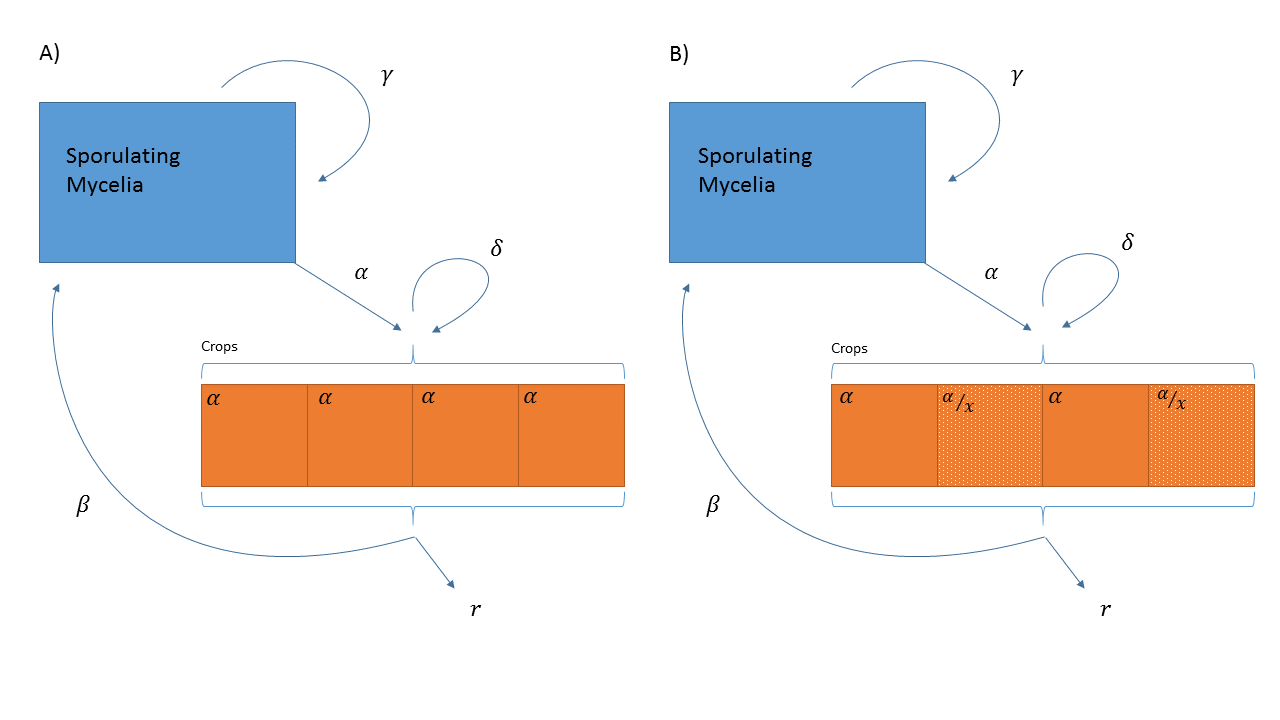
\includegraphics[width=\textwidth]{fig1}}
  \caption{\textbf{A)} Simplified system of \emph{Aspergillus flavus} infection to spatially arranged crops with assumed homogeneity in infection rates per crop. This model is best applied to a monoculture o maize. \textbf{B)} The same system with heterogeneity in crop infection rates as determined by a random $x$ coefficient. This system is best applied to modeling maize (no change in $\alpha$ value with a mixture of other crops nearby.)}
\end{figure}

\newpage

\begin{figure}[h!t]
  \noindent
  \makebox[\textwidth]{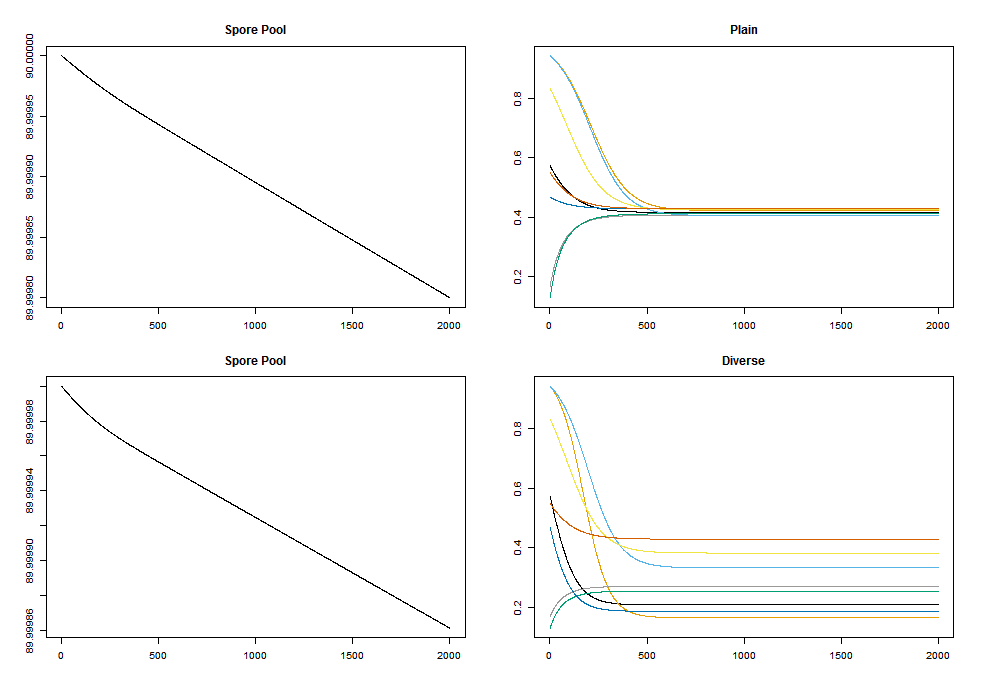
\includegraphics[width=\textwidth]{fig2}}
  \caption{Dynamics of the system after 2,000 discrete timesteps. The spore pool y-axis is discrete units of the modeled conidia of \emph{A. flavus}. The y-axis of the spatial crops are scaled to percent infection. Each crop is represented in a different color. Maize is represented as an orange line with the highest infection rate.}
\end{figure}

%------------------------------------------------------------------------------
% Appendix
%------------------------------------------------------------------------------

\newpage

\section*{\upshape\textsc{Appendix}}

\singlespacing

\begin{code}
\begin{lstlisting}[frame=single]
library('deSolve')
library('fields')
source('http://faraway.neu.edu/data/cb.R')

set.seed(2)
npops = 8
maxtime = 2000

N.R = runif(1, min=0, max=0.1)  # Crop recovery rate
N.K = runif(1, min=10, max=20)  # Crop max infections

P.K = 90   # Spore carrying capacity

N.init = runif(npops, min=0, max=N.K)
P.init = 90

solve.spatial = function (x, maxtime, alpha) {
  P = numeric(maxtime)
  P[1] = P.init

  N = matrix(nrow=maxtime, ncol=x)
  N[1, ] = N.init

  beta = max(alpha)  #
  gamma = 0.0000001 # Spore rate of growth

  for (i in 2:maxtime) {
    P[i] = P[i-1] + P[i-1] * gamma * sum(N[i-1,]) * (1 - (((P[i-1] + (beta * P[i-1] / npops)) / P.K)))

    P[P[i] <= 0 | is.nan(P[i])] = 0

    N[i,] = N[i-1,] + N[i-1,] * (- N.R) * (1 - (N[i-1,] / N.K)) + alpha * P[i-1] * (1 - (N[i-1,] / N.K))
  }
  return(list(N=N, P=P))
}

results.plain = solve.spatial(npops, maxtime, c(runif(npops - 1, min=0.0014, max=0.0015), 0.0015))
results.mixed = solve.spatial(npops, maxtime, c(runif(npops - 1, min=0.0005, max=0.0015), 0.0015))

print(max(tail(results.mixed$N, 1)[1,])/max(tail(results.plain$N, 1)[1,]))

par(mfrow=c(2, 2))
par(cex=0.6)
par(mar=c(3, 3, 3, 3), oma=c(1, 1, 1, 1))

plot(1:maxtime, results.plain$P, xlab='', ylab='', type='l', col=cb, lty=1, main='Spore Pool')
matplot(1:maxtime, results.plain$N/N.K, xlab='', ylab='', type='l', col=cb, lty=1, main='Plain')
plot(1:maxtime, results.mixed$P, xlab='Time', ylab='', type='l', col=cb, lty=1, main='Spore Pool')
matplot(1:maxtime, results.mixed$N/N.K, xlab='Time', ylab='', type='l', col=cb, lty=1, main='Diverse')


```
````{r fig.width=7, fig.height=6, warning=F, message=F}
a = 0
for (i in 1:5) {
  results.plain = solve.spatial(npops, maxtime, c(runif(npops - 1, min=0.0014, max=0.0015), 0.0015))
  results.mixed = solve.spatial(npops, maxtime, c(runif(npops - 1, min=0.0005, max=0.0015), 0.0015))
  a = a + max(tail(results.mixed$N, 1)[1,])/max(tail(results.plain$N, 1)[1,])
}
print(a/5)
\end{lstlisting}

\end{code}

%------------------------------------------------------------------------------
% Literature Cited
%------------------------------------------------------------------------------

\newpage
\singlespacing
\let\itshape\upshape     % Remove italics from Bibliography
\bibliographystyle{apacite}
\bibliography{C:/dev/latexlocal/bibliographies/aflatoxin}

\end{document}
